\documentclass[12pt]{report}
\usepackage{pck-english}
%\usepackage{algorithmicx}
%\usepackage{algorithm}
%\usepackage{algorithmic}
\usepackage{standalone}

% Default fixed font does not support bold face
\DeclareFixedFont{\ttb}{T1}{txtt}{bx}{n}{10} % for bold
\DeclareFixedFont{\ttm}{T1}{txtt}{m}{n}{10}  % for normal

% Custom colors
\usepackage{color}
\definecolor{deepblue}{rgb}{0,0,0.5}
\definecolor{deepred}{rgb}{0.6,0,0}
\definecolor{deepgreen}{rgb}{0,0.5,0}

% Python style for highlighting
\newcommand\pythonstyle{\lstset{
language=Python,
basicstyle=\ttm,
numbers=left,
numberstyle=\ttm,
%stepnumber = 1,
otherkeywords={self},             % Add keywords here
keywordstyle=\ttb\color{deepblue},
emph={MyClass,__init__},          % Custom highlighting
emphstyle=\ttb\color{deepred},    % Custom highlighting style
stringstyle=\color{deepgreen},
frame=single,                         % Any extra options here
showstringspaces=false            %
}}

% Python environment
\lstnewenvironment{python}[1][]
{
\pythonstyle
\lstset{#1}
}
{}

\newcommand\cstyle{\lstset{
language=c,
basicstyle=\ttm,
%numbers=left,
%stepnumber = 1,
otherkeywords={self,\#include,\#pragma},             % Add keywords here
keywordstyle=\ttb\color{deepblue},
emph={MyClass,__init__},          % Custom highlighting
emphstyle=\ttb\color{deepred},    % Custom highlighting style
stringstyle=\color{deepgreen},
frame=single,                         % Any extra options here
showstringspaces=false            %
}}

% Python environment
\lstnewenvironment{c_lang}[1][]
{
\cstyle
\lstset{#1}
}
{}


% Python for external files
\newcommand\pythonexternal[2][]{{
\pythonstyle
\lstinputlisting[#1]{#2}}}

% Python for inline
\newcommand\pythoninline[1]{{\pythonstyle\lstinline!#1!}}


\begin{document}

\subfile{forside.tex}

%\section*{Abstract}
%\label{sec:label}

\begin{abstract}
  I implemented a vectorized version of the KMeans algorithm using the Python library Bohrium for automatically paralellizing the operations. This allows for greater performance of the algorithm since the vectorized version is capable of running on the GPU, instead of running sequentially on the CPU. \\ \\
  Several iterations of the algorithm was implemented, one in Python, one using Numpy, and one using Bohrium. Experimental results show that difference in speeds across the three different implementations, showing how a vectorized version executes faster.
\end{abstract}


\newpage

\renewcommand{\abstractname}{Acknowledgements}
\begin{abstract}
  First of all I would like to express my sincerest gratitude to Mads B. R. Kristensen for being co-supervisor on this project, without your help and guidance the project wouldn't be the same. \\
  A special thanks to Morten Dalfoss for being my rubber duck of choice. \\
  And maybe the biggest thanks to my girlfriend Amalie Willum for never letting me go easy on anything, and always having my back when it counts.
\end{abstract}

%\section*{Acknowledgement}
%\label{sec:ackow}

\newpage

\tableofcontents

\newpage
\chapter{introduction}
\label{sec:intro}
This paper is written as part of a Bachelor project at the Niels Bohr Institute University of Copenhagen. The project deals with fast clustering of data. The author is Christopher Toft Carman. Supervised by Brian Vinter, lecturer at University of Copenhagen. Co-supervised by Mads. B. R. Kristensen bla bla bla at University of Copenhagen.
\section{Background}
\label{subsec:background}
Many disciplines in physics now a day require that use of data science to even get a result at all, thus relying on the computer to do the hard work. Thus the field of physics ``Computational Physics'' was born, where numerical analysis is used to solve the difficult physics problems. \\
The spread of 3D-scans that needs to be segmented, are used in medical image analysis, satellite images, has now gotten so big that the time requirement to process them has exceeded a practical limit, thus we need faster computers or a better way to segment the images. \\
A use case could as an example be in Plasma Dynamics simulation, where the number of particles increases exponentially, thus requiring a lot of process power. With the use of  high speed clustering, you are able to reduce the number of clusters thus keeping the number of particles at a level that can be processed. \cite{lucas}.\\
We see a lot of areas in physics that utilizes dig data, thus the performance requirement also increases, thus we must evolve the way we think about computing

\section{Goal}
\label{subsec:goal}
The goal of the project is to implement and describe the theory for a vectorized version of the unsupervised machine learning algorithm KMeans using the library Bohrium. Given a dataset the program is able to find a number of centroids that minimizes the internal squared distances to each centroid.
\section{Results}
\label{sec:intro_results}
I have developed an implementation of the KMeans algorithm written in Python using the library Bohrium, to automatically paralellize the operation with the goal of speeding up execution of the code. \\
The program supports three different ways of initializing the centroids, and different backends for running the code on the CPU or the GPU, giving the user more power of how they want to run KMeans.\\ To plot the results of the benchmarks conducted in this paper we used the library Benchpress, during the project I was able to submit several pull requests\footnote{Pull request as in git pull request to add to the codebase of the library} to both Bohrium and Benchpress. \\
All the code can be found in my github repository \href{https://www.github.com/shadesfear/bachelor}{https://www.github.com/shadesfear/bachelor}









\chapter{Theory}
\label{sec:label}

\section{K-Means}
\label{subsec:kmeans}

K-means clustering is a method developed for partitioning a set of points $X = \{x_1, x_2, ..., x_n\}$ in a d-dimensional space into a set of clusters $S = \{s_1, s_2, ..., s_k\}$, hence the name K-means. The algorithm takes n points and k number of clusters, it returns points split up into these clusters where an assignment has been made for each point to a given cluster. This problem is what is called a NP-hard problem this means that it's computationally hard. KMeans usually is one of the fastest clustering methods, but it suffers that it might converge to a local minimum instead of the sought after global minimum, but there are ways to more or less correct this fault.\cite{lloyd}

\section{Lloyd's Algorithm}
\label{subsec:lloyds}

The most common implementation of k-means is the so called Lloyd's Algorithm that uses an iterative refinement approach. To start of some initial centroids as the center of each cluster is called, is chosen at random, then at each iteration of the algorithm two steps are executed, and repeated until the individual clusters does not change anymore (This is called convergence), or is terminated by an upper bound of iterations. There are many methods for choosing the initial centroids, a common method is the Forgy method, where k random points of the input data set is chosen as the centroid. Another example is the KMeans++ method of initializing centroids, that aims to by careful seeding have a better start for the algorithm, and such reach convergence faster.\cite{plusplus} The two steps for each iteration can be outlined as such: \\

\textbf{Assignment:} For each data point, compute all distances to all centroids, and find the nearest one. assign this point to the cluster.\\
\textbf{Update:} For each cluster calculate the mean of all the assigned points to the cluster and move the cluster to the mean\\ \\

In a more strict notation it's as follow:

\begin{algorithm}[h!]
  \caption{Kmeans algorithm}
  \begin{algorithmic}

    \Procedure{Kmeans}{}
    \State $\textit{X} \gets \{x_1, x_2, .. x_n\}$
    \State $c_1, ..c_2,...,c_k \gets$ RANDOM(points, K)
    \While{not converged}
    \ForAll{ $x \in X$ }
    find $\phi_c(x)$ (closest centroids to x)
    \EndFor
    \ForAll{$c \in C$}
    $c =$ mean($\{x \in X | \phi_C(x) = c\}$)
    \EndFor
    \EndWhile
    \EndProcedure
  \end{algorithmic}

\end{algorithm}

The algorithm has some problems, it has to compute the distance from each point to each cluster in each iteration, this takes computational power. To compute the distance between two points $p,q \in \mathbb{R}^d$ we have to do the following computation:

\begin{equation}
  L = ||p - q||^2 = (p_1 - q_1)^2 +...+(p_d - q_d)^2
\end{equation}
This is known as the euclidian distance, this can be written more compactly as

\begin{equation}
  L = \sqrt{\sum_{i=1}^d(p_i - q_i)^2}
\end{equation}
This gives d subtractions, d multiplications and d-1 sums, and then for comparison with the previous cluster calculate the following: $d_{min} > d$ \\
This evaluates to $3\cdot d$ calculations for each point and cluster. Thus for each iteration we would need to execute $3d \cdot n \cdot k$ operations.

\section{Convergence}
\label{subsec:Convergens}
The algorithm is said to have converged when the assignment of cluster no longer changes, there are several ways of actually determining when this convergens actually has happened. A common way of doing this is stopping when the difference of the current centroids with the centroids from the previous step of the algorithm has decreased to under some threshold $\epsilon$, this is the way that is implemented in the popular Python Library Numpy, and also the method that we will be using. \\\\
Another method is stopping whenever the labels for each centroid to their corresponding points no longer changes, this way it can be proven that it wont actually converge



\section{KMeans++}
\label{sec:plusplus}
When we initialize the clusters randomly, we don't know how well the clusters represent the optimal clusters that we are trying to find in the end, this may in some cases lead to some  bad centroids that takes a very long time to converge to til global minimum. Instead we want to use another method for initializing the centroids. For this purpose the kmeans++ algorithm was developed in 2007 by David Arthur and Sergei Vassilvitskii \cite{plusplus}.
First we let $D(x)$ denote the shortest (euclidean) distance from a data point $x$ to the closest centroids that we have already chosen. And we also define a probability as the following:
\begin{equation}
P(x) = \frac{D(x)^2}{\sum_{x\in X}D(x)^2}
\end{equation}
Then the algorithm is explained as such:
\begin{itemize}
  \item Take one center $c_1$ chosen at random from the set of points $X$
  \item Take a new center $c_i$ choosing $x\in X$ with probability $P(x)$.
  \item Repeat until we have k centers.
  \item Continue with normal KMeans
\end{itemize}

Here I have just pasted some of the original experimental results that David and Sergei found in their original paper.

\begin{table}[h!]
  \centering
    \begin{tabular}{|c| c |c| c| }
      & Average $\phi$ & Minimum $\phi$ & Average time (Seconds) \\
      k & Random KMeans++ & Random KMeans++ & Random KMeans++ \\
      \hline
      2&3&  ell8 & cell9
    \end{tabular}
    \caption{Table of results from original KMeans++ Paper.}
    \label{table:kpp}
\end{table}

The faster times the results show comes from the fact that with proper initialization of the centroids we reach convergence faster than with random initialized centroids. As discussed in \ref{subsec:lloyds} each iteration of the algorithm will need $3d \cdot n\cdot k$ operations, so decreasing the number of iterations will have a huge impact on performance.

\section{Numpy}
\label{sec:numpy}
NumPy is a math library for python, that adds support for large matrix operations in any dimension, with support for higher level operations. NumPy adds support for array programming that we will utilize greatly in this project, this also means that we will have to write less code and use easier syntax that lets the programmer focus on creating software and not understating complex syntax.
\subsection{Broadcasting}
\label{subsec:Broadcasting}

On of the more advanced features of NumPy that we utilize in this project is broadcasting, broadcasting is NumPy's way of adding, subtracting or any other arithmetic on arrays of different sizes. Basically NumPy duplicates the smaller array such that the size and dimension of the smaller array matches the bigger array. A basic example of how this is handled can be seen in figure \ref{fig:broadcasting}.

\begin{figure}[H]
  \centering
  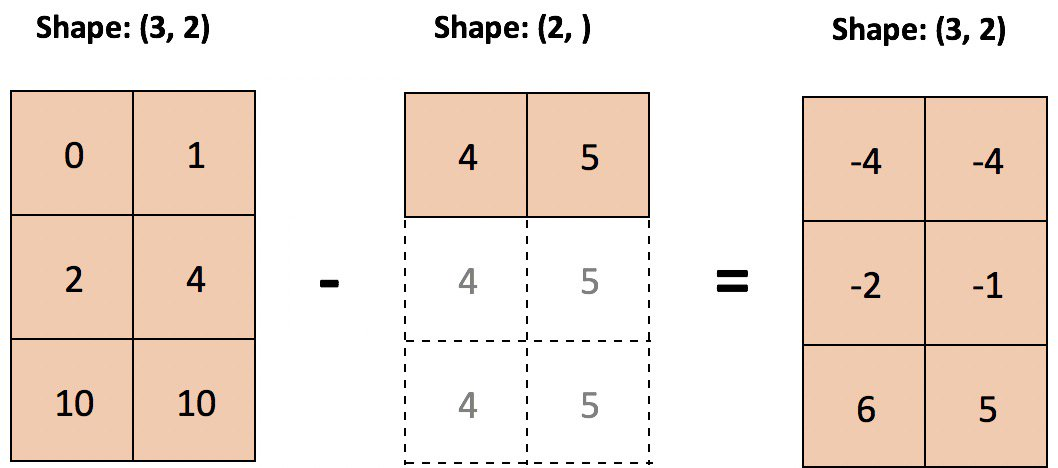
\includegraphics[width = 0.6\textwidth]{images/broadcasting.png}
  \caption{An example of how NumPy broadcasting works.\label{fig:broadcasting}}
\end{figure}





\section{Bohrium}
\label{subsec:Bohrium}
Bohrium is framework that aims to present a way to speed-up array programming, it's a modular framework with support for multiple alternate front end and back ends. Bohrium was created in 2013, by Mads R. B. Kristensen, this makes it possible to both run code on the CPU (Using OpenMP) or the GPU (Using Cuda / OpenCL) and all of this is done without explicitly writing any code for the different platforms.

\subsection{How it works}
\label{subsec:hiw}
Bohrium lazily record any array operations that is used, this could as an example be from NumPy, and turn them into bytecode instruction set. An overview can be seen in figure \ref{fig:bohrium_overview}. Bohrium also utilizes lazy CPU / GPU communication which means that Bohrium only moves data between the CPU and the GPU when the data is accessed directly by Python Code \cite{bohrium_website}

\begin{figure}[H]
  \centering
  \documentclass{standalone}
\usepackage{tikz}
\begin{document}

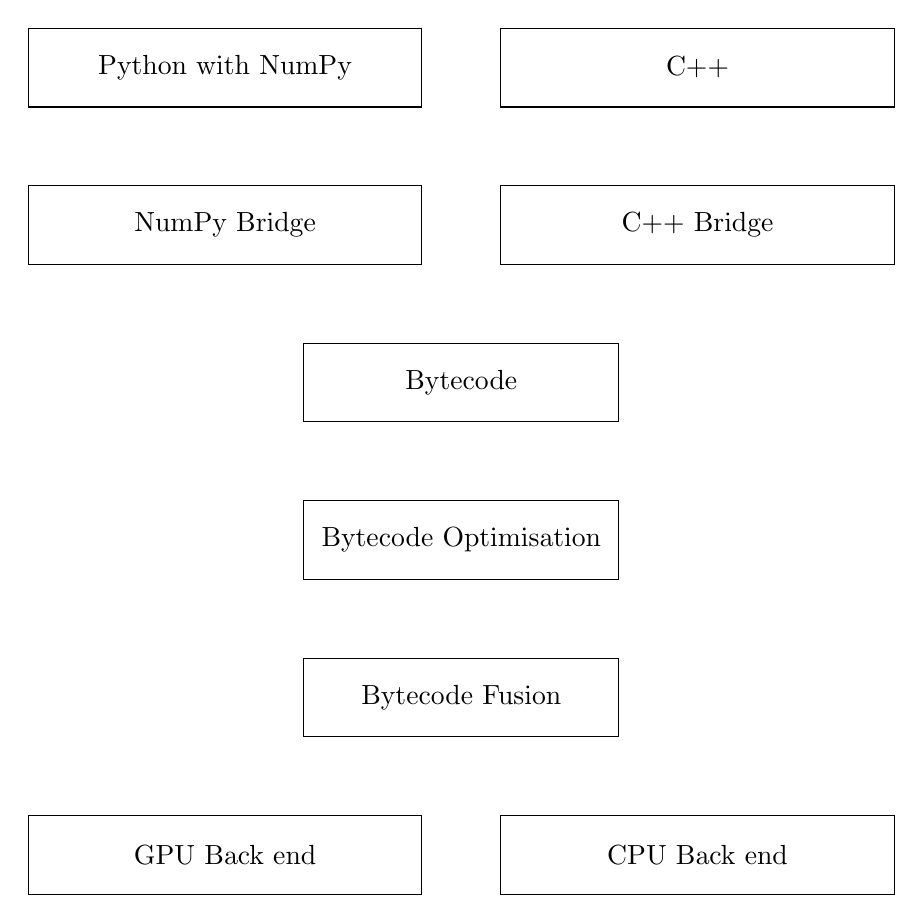
\begin{tikzpicture}
  \draw (1.5,0) rectangle (6.5, 1) node[pos=.5] {Python with NumPy};
  \draw (7.5,0) rectangle (12.5, 1) node[pos=.5] {C++};
  \draw (1.5,-1) rectangle (6.5, -2) node[pos=.5] {NumPy Bridge};
  \draw (7.5,-1) rectangle (12.5, -2) node[pos=.5] {C++ Bridge};

  \draw (5,-3) rectangle (9, -4) node[pos=.5] {Bytecode};
  \draw (5,-5) rectangle (9, -6) node[pos=.5] {Bytecode Optimisation};
  \draw (5,-7) rectangle (9, -8) node[pos=.5] {Bytecode Fusion};

  \draw (1.5,-9) rectangle (6.5, -10) node[pos=.5] {GPU Back end};
  \draw (7.5,-9) rectangle (12.5, -10) node[pos=.5] {CPU Back end};

\end{tikzpicture}

\end{document}

\caption{\label{fig:bohrium_overview}The components that Bohrium are made out of}
\end{figure}

\section{Vectorization}
\label{subsec:vectorization}

The point of vectorization is to generalize operations on scalars to apply on vectors, matrices and also higher-dimensional arrays. The idea is to do operations on an entire set of values instead of each single item in the set. As en example the operation of adding two arrays together in a scalar function would look like this implemented in python
\begin{lstlisting}[language=C]
  for (i=0; i < n; i++)
      for (j = 0; j < n; j++)
          a[index_a][index_b] += b[index_a][index_b]
\end{lstlisting}

This tedious way of coding can now be abstracted away, as more and more programming languages and libraries support what is known as array programming, as an example in the library for python called Numpy the code for adding to vectors together can the trivialized to $a + b = c$ this leads to simpler code and it makes it possible for the programmer to speak the same language as mathematicians.

Vectorized operations are typically allows for the operations to be run in parallel, thus speeding up the operation time. This in turn allows us further to run our code on GPU's which should lead to even greater speedups. These speedups will be discussed en greater detail when we discuss my vectorized implementation of the KMeans algorithm and my results.

\section{OpenMP}
\label{subsec:openmp}
OpenMP is  library that supports what is known as shared memory multiproccesing. So when programming inside the framework of OpenMP all of the threads utilize the same memory and data. With OpenMP it's easy to paralellize code on the CPU, just by adding a pragma to the code. An example of this could to automatically try to paralellize a for loop as seen in listing \ref{code:openmp}

% \begin{lstlisting}[language=C, caption={How to automatically paralellize for loop with OpenMP.}]
%   #include <omp.h>
%   #pragma omp paralellize for
%   for (i=0; i < n; i++)
%       ....
% \end{lstlisting}

\begin{c_lang}[caption={Example of how to automatically paralellize for loops with OpenMP}\label{code:openmp}]
  #include <omp.h>
  #pragma omp paralellize for
  for (int i=0; i < n; i++) {
    ....
  }
\end{c_lang}

\section{OpenCL}
\label{subsec:opencl}
OpenCL is a programming framework for writing parallel code on CPUs, GPUs, clusters etc, doing so by writing in the language ``OpenCL C'' this allows us to run user-kernels (Code to be run on GPU device) on the GPU with the purpose of getting greater speedups of the code. One of the first examples you see of OpenCL is the vector addition as seen in \ref{code:opencl}, consider this to be the Hello World of OpenCL.

\begin{c_lang}[caption={Example of adding to vectors in OpenCL}\label{code:opencl}]
  #pragma OPENCL EXTENSION cl_khr_fp64 : enable
  kernel void vecAdd(global double *a, global double *b,
                                       global double *c){
    int id = get_global_id(0);
    c[id] = a[id] + b[id];
  }
\end{c_lang}



\chapter{Implementation}
\label{subsec:implement}
\section{Overview}
\label{subsec:overview}
The program that was developed is aptly named Bohrium Kmeans, and as discussed is developed in Python using the Bohrium library for automatic GPU acceleration created by Mads. R. B. Kristensen. Bohrium Kmeans as most other kmeans implementations takes a set of points in any number of dimensions and number of clusters, this means that there is a large overlap in the way to use Bohrium Kmeans compared to some of the more popular libraries such as SKlearn for Python.\\
Bohrium Kmeans allows for alot of different parameters to be changed, as a concequence the user has control of how they want to use the program as an example they have the ability to choose how to initialize centroids, either by k-random centroids, first k-points or by the described kmeans++ algorithm.\\
In the following chapter I will desribe and detail some of the ways I implemented the algorithm and a chronological order and the issues and solutions i combated.
\section{Try: Python}
\label{subsec:beginning}
To start of with the goal was to implement a barebones version of the kmeans algorithm in python without use of any external libraries, this decision means that we will have no array programming or vectorization. So we are left with only our knowledge of programming and a blank editor.
This means that we are forced to use loops in python, luckily python includes the feature: list comprehension which is a way of creating new list from  old list depending on some condition. This can get rid of some larger loops and as a bonus list comprehension is optimized for the python interpreter, just take a look this example where we choose k centroids from the set of points, first with a loop the standard way where we have to initialize the list to store the centroids in first, and then with a list comprehension.

% \begin{lstlisting}[language=Python]
%   centroids = []
%   for i in range(k):
%       centroids.append(points[randint(0, len(data)-1)])
%     \end{lstlisting}
\begin{python}[caption={Generating k random centroids using for loop in python}]
  centroids = []
  for i in range(k):
      centroids.append(points[randint(0, len(data)-1)])
\end{python}
Now with list comprehension
% \begin{lstlisting}[language=Python]
% centroids = [points[randint(0, len(data)-1)] for i in range(k)]
% \end{lstlisting}

\begin{python}
centroids = [points[randint(0, len(data)-1)] for i in range(k)]
\end{python}

One way or the other we still loop sequentially k times and doing it this way is not a vectorized approach thus we cannot hope to accelerate it in any meaningful way. A vectorized version will be discussed in the next chapter where start discussing the basic implementation using Numpy. \\
Another maybe even more surprising example, is the assignment step of Lloyd's algorithm where we have to compute the distance from each point to each centroid, without any vectorization we are again forced to use for loops, but this time a nested one

% \begin{lstlisting}[language=Python]
%   for p_idx, point in enumerate(points):
%       distance_array = [0] * k #Initialize empty array
%       for c_idx, centroids in enumerate(centroids):
%           distance = euclidean_distance(point, centroid)
%           distance_array[c_idx] = distance
%       labels[p_idx] = distance_array.index(min(distance_array))
%     \end{lstlisting}

\begin{python}[caption={Python example of calculating the distances between each centroid and each point. Lastly getting the label for each point for which centroid they belong to.}]
  for p_idx, point in enumerate(points):
      distance_array = [0] * k #Initialize empty array
      for c_idx, centroids in enumerate(centroids):
          distance = euclidean_distance(point, centroid)
          distance_array[c_idx] = distance
      labels[p_idx] = distance_array.index(min(distance_array))
\end{python}

This is definitely hurtful for performance as we have to execute the body of the loop $n \times k$ times (not to mention the loop in the euclidean distance function)



\newpage
\section{Except: Numpy}
\label{subsec:middle}
Now we turn our heads to a version written with the help of the library NumPy, NumPy allows us to utilize array programming as already discussed. This makes it so that we can carry out array operations with simple instructions and then NumPy will take the instructions and carry them out in a much more optimized way. Let us take a quick look at the previous code snippet where we chose $k$ random centroids, but this time using NumPy

% \begin{lstlisting}[language=Python]
% import numpy as np
% row_i = np.random.choice(points.shape[0], k)
% centroids=points[row_i,:]
% \end{lstlisting}

\begin{python}[caption = {Choosing k random centroids using NumPy.}\label{code:numpykrandom}]
import numpy as np
row_i = np.random.choice(points.shape[0], k)
centroids=points[row_i,:]
\end{python}

This let's NumPy handle all the dirty work and should in theory give better performance, lets just take a quick look at what speedups we might expect. We performed a test with the previous code snippets discussed for choosing k random centroids from a set of points. The results can be seen in figure \ref{fig:numpyvspython}, the speedups from choosing 5000 centroids is about 13 times faster when going from Python to NumPy, we could expect to see even greater results when going to larger values of $k$.

\begin{figure} [H]
  \centering
  \includegraphics[width=0.9\linewidth]{images/pybnumpy.pdf}
  \caption{Benchmark of choosing k random centroids from a set of points, first using list comprehension in python, then with NumPy. The number of centroids chosen is \{10, 20, 50, 100, 1000, 5000\}}
  \label{fig:numpyvspython}
\end{figure}

So in order to minimize time spent on computation we should utilize NumPy's array programming whenever possible, this means in some cases rewriting code that seemingly seems fast and correct just to push some small gains in performance.
As discussed in section \ref{subsec:lloyds} Lloyd's algorithm will for each iteration need $3d \cdot n \cdot k$ operations to calculate the Euclidean distance between two points, so this will indeed a focus point to vectorize, where we are also able to make us of some of NumPy's more advanced features such as broadcasting to implement a faster vectorized version, lets take a look at an example in algorithm \ref{alg:eucdist}. As we see there are now no for loops to deal with and once the special features of NumPy is grasped the notation is also much simpler.

% \begin{algorithm}
%   \caption{Euclid’s algorithm}
%   \label{euclid}
%   \begin{algorithmic}[1]
%     \Procedure{Euclid}{$a,b$}
%     \Comment{The g.c.d. of a and b}
%     \State $r\gets a\bmod b$
%     \While{$r\not=0$}
%     \Comment{We have the answer if r is 0}
%     \State $a\gets b$
%     \State $b\gets r$
%     \State $r\gets a\bmod b$
%     \EndWhile
%     \label{euclidendwhile}
%     \State \textbf{return} $b$
%     \Comment{The gcd is b}
%     \EndProcedure
%   \end{algorithmic}
% \end{algorithm}

\begin{algorithm}
  \caption{Euclidean Distance Numpy}
  \label{alg:eucdist}
  \begin{algorithmic}[1]
    \Procedure{$EUC\_DISTANCE$}{Points, centroids}
    \State $X \gets $ points - centroids$[:,None]$
    \Comment{Numpy Broadcasting}
    \State Distances $\gets np.sqrt(X * X).sum(2)$
    \EndProcedure
  \end{algorithmic}
\end{algorithm}

In the second step of the kmeans algorithm we have to move the centroids, using a seemingly naive approach this would take two for loops taking around a running time of $k^2$ times to complete. This can be seen in algorithm \ref{alg:movecent}, and then a fast vectorized approach again using some advanced NumPy features to rid ourselves of loops can be seen in code snippet \ref{code:movecent}, our gain in speeds when going from the sequential to vectorized approach will be discussed in more detail in the results section, also the evolution of listing \ref{code:movecent} will be discussed in the next section.


\begin{algorithm}
  \caption{Move Centroids}
  \label{alg:movecent}
  \begin{algorithmic}[1]
    \Procedure{$move\_centroids$}{}
    \For{$i \gets 0, k$}
    \ForAll{points belonging to centroid $i$}
    \State $sum \gets sum + points$
    \EndFor
    \State centroid[i] = sum / len(sum)
    \EndFor
    \EndProcedure
  \end{algorithmic}
\end{algorithm}



\begin{python}[caption={Numpy Vectorized version of move centroids}\label{code:movecent}]
import numpy as np
def move_centroids(points, closest, centroids, k):
    mask = (labels == np.arange(k)[:,None])
    return mask.dot(points)/ mask.sum(1)[:,None]
\end{python}

\newpage

\section{Finally: Bohrium}
\label{subsec:finally}
Let us now turn our heads to the final beast that is Bohrium, automated acceleration of our matrix operations sounds awesome, just replace the import of NumPy, with an import of Bohrium in our previous code and all the code should work, super fast kmeans right? Not so fast, not all NumPy function's have been implemented in Bohrium yet, and some are just not able to be accelerated, then we have two choices going forward, either find another way to rewrite the code such that Bohrium can automatically accelerate it, or write a custom userkernel for you problem in either OpenMP or OpenCL. In my efforts to create a version using Bohrium, I have resorted to both methods, sometimes going back and forth when my own knowledge of the problem expanded, thus rewriting and refactoring the same code multiple times getting a better and better implementation, the gain in performance when going to Bohrium will be discussed in detail in the next chapter.
\subsection{Initialize the centroids}
\label{subsec:userkernel}
Let's take a look at a problem that was not implemented in Bohrium, the simple task at the start of running the kmeans algorithm is initializing centroids. To initialize k random centroids as described in listing \ref{code:numpykrandom} unfortionatly this does not work in Bohrium and will resort to using NumPy that can not be parallelized. So we write c code to shuffle an array and we can pick the first k elements to initialize the centroids. To do this we implemented Fisher-Yates shuffle that was popularized in Donald Knuths book ``The Art of computer Programming'', the algorithm is described in listing \ref{code:fisheryates}, the only difference that my version shuffles along the first dimension of the array, the code can of course be seen in the \href{https://github.com/shadesfear/bachelor}{repository}

\begin{algorithm}
  \caption{Shuffle an array a of n element}
  \label{code:fisheryates}
  \begin{algorithmic}[1]
    \Procedure{fisher\_yates}{}
    \For{i \textbf{from} n-1 \textbf{downto} 1}
    \State $j \gets$ random integer such that $0\leq j \leq i$
    \State swap a[$i$] and a[$j$]
    \EndFor
    \EndProcedure
  \end{algorithmic}
\end{algorithm}

\subsection{Reasign the centroids}
\label{subsec:reasign}
This first naive solution i implemented worked in NumPy using a for loop in a list comprehension displayed in algorithm \ref{code:reasign_naive} as we know, for loops in python are slow and we are not able to easily paralellize the code. So we must find another way either by writing a userkernel or finding another way using only functions that actually are implemented in Bohrium. My first attempts was to write my own userkernel using OpenMP than can run on the CPU \\

% \begin{algorithm}
%   \caption{Reasign centroids (naive)}
%   \label{code:reasign_naive}
%   \begin{algorithmic}[1]
%     \Procedure{}{}
%     \
%     \EndProcedure

%   \end{algorithmic}
%\end{algorithm}
\begin{python}[caption={Naive implementation of reassigning the centroids using for loop }\label{code:reasign_naive}]
  import bohrium as bh
  new_centroids = bh.array([points[closest==k].mean(axis = 0)
                                    for k in range(self.k)])
\end{python}

The userkernel follows the pattern of algorithm in \ref{alg:movecent}, thus we using some \textbf{for} loops that in OpenMP we parallelize with the \#pragma discussed in \ref{subsec:openmp}

\section{Why  Not Kmeans++?}
\label{sec:notplusplus}
I Told you that we would not be using Kmeans++ for initializing the centroids, now im going to tell you why. KMeans++ is not really suited for running in parallel as a result of it's sequential nature it scales badly with greater values of $k$, do the way it works, where the next centroid chosen depends on the last one. This was the subject of the 2012 paper ``Scalable Kmeans++'' \cite{scalableKmeans} written by Bahman Bahmani, Benjamin Moseley, Andrea Vattani, Ravi Kumar, Sergei Vassilvitskiil, where they were tasked to implement a scalable and parallel version of the KMeans$++$ algorithm, this was not a possibility to implement as of the writing of this paper, but may be subject to further investigation.




\chapter{Results}
\label{sec:label}
In this chapter I will try to provide the reader with acceptable proof that we did indeed gain an increase in performance when going from plain Python to Bohrium. This was done by performing different benchmarks of the different implementations of the KMeans algorithm, for different number of points, in different number of dimensions (features) and in different number of centroids (k).\\\\ The benchmarks was conducted using the Python library Benchpress that is also created by Mads B. R Kristensen that makes it a breeze to create soffisticated Benchmarks of different sizes and functions by creating a suite file that describes the functions to run with different parameters, and then executing them one by one.\\
For the benchmarks we will use the same method of initialization for all the different benchmarks namely random initialization with the same seed such that the randomness is predictable.


\section{Python VS Bohrium}
\label{sec:pyvbohrium}
Now we will explore the increases in performance in pure Python compared to my version in Bohrium, when running on the CPU. First I will explore runtimes of the algorithm for an increasing number of random points with the same seed to make sure that the benchmark across runs are fair, then I will conduct the benchmark for an increasing number of values for $k$, with a fixed number of random points. This results are seen in figure \ref{fig:pythonvsbohrium}, as we see, bohrium is faster and scales much better, allowing for larger datasets in a shorter time.

\begin{figure}[H]
  \centering
  \includegraphics[width=0.9\linewidth]{images/python_vs_bohrium1.pdf}
  \caption{\label{fig:pythonvsbohrium}Runtimes of the KMeans algorithm run on a varying number of points, the notation reads ``multiplier*exponent'', such that Bohrium/5*5 is KMeans using Bohrium with $5*10^5$ number of points, the number of centroids was fixed to be 25. \textbf{LOWER IS BETTER}}
\end{figure}

\section{NumPy VS Bohrium}
\label{sec:numpyvsbohrium}
In this section we will look at the performance in  running my implementation of the KMeans algorithm in  NumPy vs Bohrium, we will do the same as in the last section, first looking at performance for different number of points, and then we will be looking at different number of centroids. Again we expected to see a gain in performance, and that is what we got, although less than in the previous example.

\begin{figure}[H]
  \centering
  \includegraphics[width=0.9\textwidth]{images/numpy_vs_bohrium_points.pdf}
  \caption{\label{fig:label}Runtimes of Kmeans implemented in Bohrium VS NumPy with a varying number of points. \textbf{LOWER IS BETTER}. The notation reads that ``times*exponent'' such that 3*5 means $3 \times 10^5$ number of points}
\end{figure}


\begin{figure}[H]
  \centering
  \includegraphics[width=0.9\linewidth]{images/bohr-numpy-kmeans2.pdf}
  \caption{\label{fig:bohriumvsnumpy}Benchmark of the kmeans algorithm of the same dataset with different number of centroids. The centroids chosen is \{10, 20, 30, 40, 50, 100, 500\}}
\end{figure}



\section{CPU vs GPU}
\label{sec:cpugpu}
When comparing speeds on the CPU compared to the GPU we conduct the test on the machine Nelson, provided by the NBI this machine is equipped with the Nvidia 680 graphics card, although not the fastest and newest card on the market today, it should provide us with ample computing power for our purposes. I conducted two experiments, first one is only running the Euclidean distance algorithm on to different sets of points that are randomly generated with increasing number of points for each iteration of the benchmark. The results are depicted in figure \ref{fig:points2}. The Euclidean distance algorithm was written completely in Bohrium, so no userkernels are written for this function, thus the increase in performance is purely from automated parallelization of the code.

\begin{figure}[ht]
  \centering
  \includegraphics[width=\textwidth]{images/euc_function_points2.pdf}
  \caption{\label{fig:points2}Six runs of the Euclidean Distance algorithm, running three times on the CPU, then three times on the GPU with varying number if points in each set.}
\end{figure}
The second experiment that i chose to run is the assignment step of the KMeans algorithm with varying number of centroids $k$, for this step I have written my own userkernel, as a result of this the gain speed from going from the CPU to the GPU is my own manual paralellization of the code first on the CPU using OpenMP and then on the graphics card using OpenCL. The results are portrayed in figure \ref{fig:k5}, the reason for not running the full KMeans algorithm on the graphics card is that the reassignment step of the KMeans algorithm written in pure Bohrium, does not run well on Nelson, this seems to be a bug in how to function are implemented in Bohrium, and the time scope of the project did not allow me to write my own userkernel for the purpose.

\begin{figure}[ht]
  \centering
  \includegraphics[width=\textwidth]{images/cpugpu_k5.pdf}
  \caption{\label{fig:k5} Histogram depicting ten runs of the assignment step of the KMeans algorithm, five times on the CPU, then 5 times on the GPU, each with a varying number of centroids}
\end{figure}






\chapter{Experiments}
\label{sec:experi}
In this chapter i will discuss two common use cases for the KMeans algorithm, the first example is where we try to find groups or clusters in data from heart patients. The other example is where we try segment a CT scan of the brain, the idea is to reveal similar attributes in the image for further image analysis. These experiments was conducted in Jupyter Notebooks, as it's a nice way to visualize data processing, the notebooks can be found in the github \href{https://github.com/shadesfear/bachelor}{repository}, but images will also be presented laters in this chapter.
\section{Heart Disease}
\label{sec:heart}
The setup of the experiment is that we want to find groups in the data of heart patients, the data can be found at this \href{https://www.kaggle.com/ronitf/heart-disease-uci}{link}. The dataset contains 14 different features (or dimensions) relating to the health of heart, in which the last feature is the ``target'' or if the person has actually gotten a major heart disease or not. The plan is then:
\begin{enumerate}
\item Deal with non numerical data
\item Perform KMeans clustering on the dataset minus the target feature
\item Check how ``correct'' our clustering is
\end{enumerate}
To deal with the non numerical data, we encode each unique value of the coloum with a value, as an example from our dataset we map ``male''/``female'' to either 1 and 0 or 0 and 1.\\
Performing KMeans on the dataset was a trivial task, we set the number centroids to two, to try and find binary structure in the data. Since we then get a label for each thirteen dimensional point in the dataset we check the overlap from the target coloumn versus our labels. This revealed an overlap of about 43\% or 57\%, \textbf{EXPLAIN WHAT IT MEANS}, these seemingly bad values does have an explaination, we did not normalize our dataset, as we are using an Euclidean distance metric for comparision if the data is not normalized we will not get good values \cite{kmeansconvergence}. After normalizing we now get 81\% or 21\% overlap, but better! Now these labels can used as a feature in lets say a logistical regression.
\subsection{Image Segmentation}
\label{subsec:imgseg}
Another classic example is image segmentation, the task is to cluster the image into groups based on similar features, this could as an example be the RGB color value of each pixle that we might want to group together. In my attempt at image segmentation I looked at grey scale values of a CT scan of a human head, in the hopes that we might find underlying structures such as bones and not bones, in lack of a better term. The image before and after segmentation can be seen in figure \ref{fig:imgseg}

\begin{figure}[h]
    \centering
    \begin{subfigure}[t]{0.5\textwidth}
        \centering
        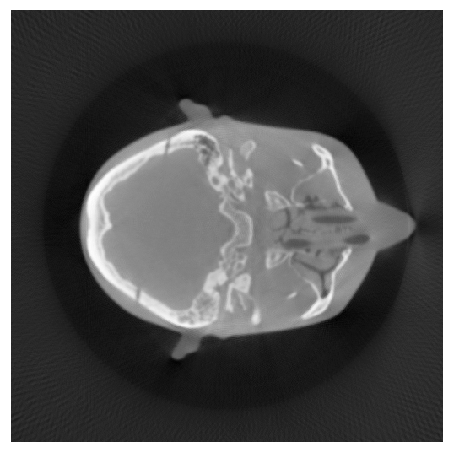
\includegraphics[width=0.9\textwidth]{images/brain512.png}
        \caption{Original image that needs to be clustered }
    \end{subfigure}%
    ~
    \begin{subfigure}[t]{0.5\textwidth}
        \centering
        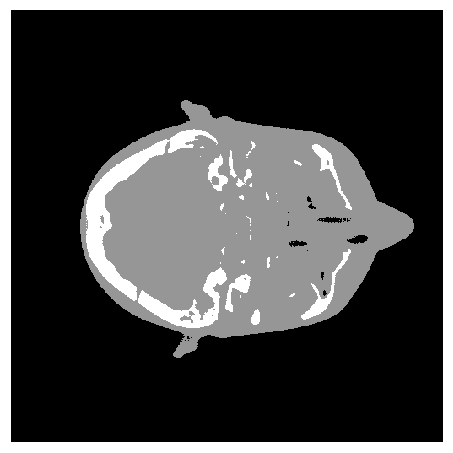
\includegraphics[width=0.9\textwidth]{images/clustering512.png}
        \caption{Image after clustering}
    \end{subfigure}
    \caption{Two images, one of the original image, and one after running the kmeans clustering with k=3}
\end{figure}
To validate the segmentation one should really calculate the Jaccard Index or Jaccard similarity coefficient, that basically is a measure of how much two sets are overlapping \cite{jaccard}. Which is basically how we validated the other experiment, the difference is that the Jaccard coefficient is just a more general version of the straight overlap of two sets.  The Jaccard coefficient is given by
\begin{equation}
J(A,B) = \frac{|A\cap B|}{|A|+|B|-|A\cap B|}
\end{equation}
Where A, and B are the two sets what we want to find the overlap of, and $0\leq J(A,B) \leq 1$. So for our experiment the two sets that we need to find overlap of is A: Our labels after clustering and B: the ``true'' labels. How does one find the True labels the reader might be inclined to ask, well since the image that we used is a generated one, we already know the labels pr default! I wont go into much detail about the calculation, but it can of course be found in the github repository. The Jaccard index of each cluster was found to be x and x and x and. This way we can see that our algorithm works decently.



\chapter{Conclusion}
\label{sec:label}
I have implemented a version of the KMeans algorithm that can run on both the CPU and the GPU using the library Bohrium for automatic acceleration of the code. My version is implemented as described in the section about implementation. The program utilizes array programming as a way of telling Bohrium how to accelerate each operation, this is done by rewriting all code to array programming, and if not possible then our have written my own userkernel to manually parallelize the code. \\
I have implemented three different version of the KMeans, one using only Python, one using only Numpy and finally one using only Bohrium with the goal of measuring the increase in performance when running code in parallel. The goal of the project was to implement a version of the KMeans clustering algorithm in bohrium such performance heavy tasks such as image segmentation can be sped up, this goal has been met. Although we cannot guarantee an increase in performance as this is hardware dependent so highly individual of the environment that you are running the program in. \\
Comparing my program to an implementation in either python or NumPy, my version does see better performance as in we see faster execution time of my implementation with the same tolerance for convergence. \\ \\

I future update for the program is to implement the Elkan's Algorithm that uses triangle inequality to avoid many distance calculations that LLoyds algorithm calculates, although much faster it uses much more memory compared to Lloyds, thus not suited for large datasets that needs clustering.


\newpage
\bibliographystyle{plain}
\bibliography{ref}

\end{document}
